\section{Utente Non Autenticato}

Di seguito vengono elencati i casi d'uso per l'utente non autenticato.

\subsection{Casi d'uso}

\subsubsection{UC-U0}

    \begin{figure}[H]
      \begin{center}
        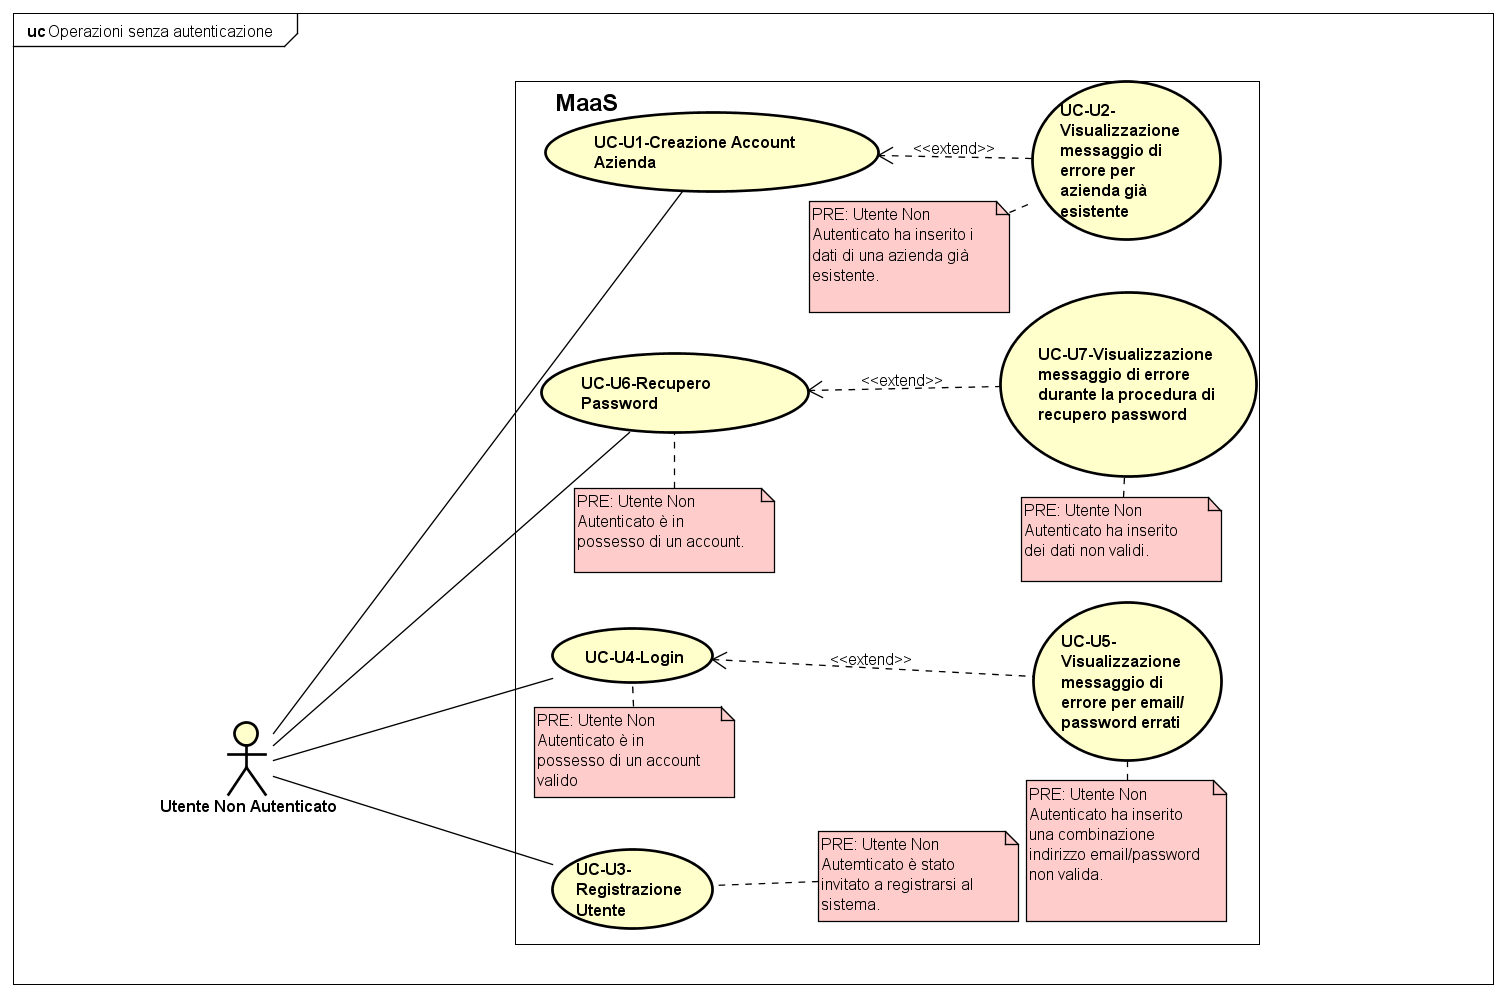
\includegraphics[width=12cm]{res/img/UCUtenti/UCUtenteNA/UC-U0-OperazioniSenzaAutenticazione_0}
      \caption{UC-U0 - Operazioni dell'utente non autenticato}
      \end{center} 
    \end{figure}    
    
    %Tabella 
    \begin{center}
      \bgroup
      \def\arraystretch{1.8}     
      \begin{longtable}{  p{3.5cm} | p{8cm} } 
        
        \hline
        \multicolumn{2}{ | c | }{ \cellcolor[gray]{0.9} \textbf{UC-U0 - Operazioni dell'utente non autenticato}} \\ 
        \hline
        
        \textbf{Attori Primari} & Utente non autenticato \\ 
        \textbf{Scopo e Descrizione} & L’utente non autenticato può creare un nuovo account per la propria azienda e registrarsi a MaaS, oppure effettuare la registrazione dopo aver ricevuto un invito. Può effettuare il login e il recupero della propria password. \\ 
        
        \textbf{Precondizioni}  & L’applicazione MaaS è funzionante e pronta all’utilizzo.
        
        Il sistema mostra all’utente non autenticato la pagina principale fornendo le funzionalità di autenticazione, registrazione e recupero password. \\ 
        
        \textbf{Postcondizioni} & L'applicazione ha eseguito le richieste dell'utente. \\ 
        \textbf{Flusso Principale} & 1. L'utente non autenticato crea un account per la propria azienda e si registra a MaaS come proprietario (UC-U1)
        
2. L'utente non autenticato riceve un invito per registrarsi a MaaS (UC-U3)

3. L'utente non autenticato in possesso di un account  effettua il login (UC-U4)

4. L'utente non autenticato può richiedere il recupero della password (UC-U6) \\
        \textbf{Estensioni} & 1. L'utente non autenticato visualizza un messaggio di errore dovuto all'inserimento di dati di un'azienda già esistente (UC-U2)
        
2. L'utente non autenticato visualizza un messaggio d'errore durante il login dovuto all'inserimento di un indirizzo email/password non corretti (UC-U5)

3. L'utente non autenticato visualizza un messaggio d'errore durante la procedura di recupero password (UC-U7)  \\
        \textbf{Inclusioni} & Nessuna \\ 
      \end{longtable}
      \egroup
    \end{center} 
    
\subsubsection{UC-U1}

    \begin{figure}[H]
      \begin{center}
        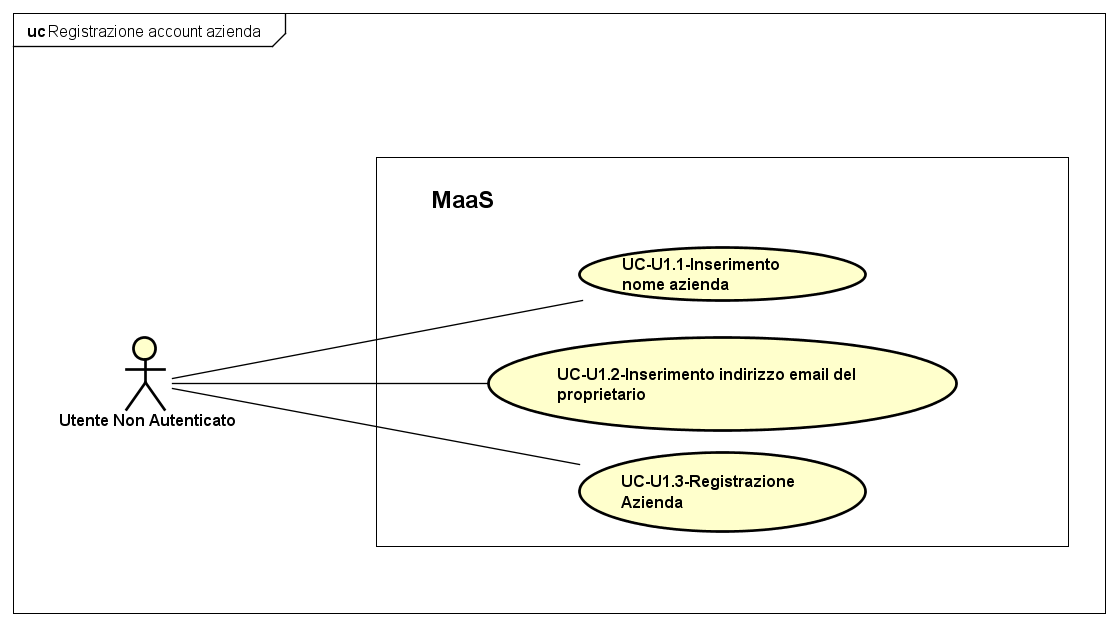
\includegraphics[width=12cm]{res/img/UCUtenti/UCUtenteNA/UC-U1-Creazione Account Azienda/UC-U1-CreazioneAccountAzienda}
      \caption{UC-U1 - Creazione account di un'azienda}
      \end{center} 
    \end{figure}    
    
    %Tabella 
    \begin{center}
      \bgroup
      \def\arraystretch{1.8}     
      \begin{longtable}{  p{3.5cm} | p{8cm} } 
        
        \hline
        \multicolumn{2}{ | c | }{ \cellcolor[gray]{0.9} \textbf{UC-U1 - Creazione account di un'azienda}} \\ 
        \hline
        
        \textbf{Attori Primari} & Utente non autenticato \\ 
        \textbf{Scopo e Descrizione} & L'utente non autenticato può creare un account per la propria azienda, inserendo i seguenti dati: nome dell'azienda, indirizzo email del proprietario e una password. \\ 
        
        \textbf{Precondizioni}  & L’applicazione MaaS è funzionante e pronta all’utilizzo.
        
Il sistema presenta all'utente la pagina di registrazione per un'azienda. \\ 
        
        \textbf{Postcondizioni} & Un'azienda è stata registrata presso MaaS e l'utente non autenticato ne è divenuto il proprietario. \\ 
        \textbf{Flusso Principale} & 1. L'utente non autenticato inserisce il nome della propria azienda (UC-U1.1)
        
2. L'utente non autenticato inserisce il proprio indirizzo email (UC-U1.2)

3. L'utente non autenticato inserisce una password e l'azienda viene registrata (UC-U1.3) \\
        \textbf{Estensioni} & Nessuna  \\
        \textbf{Inclusioni} & Nessuna \\
      \end{longtable}
      \egroup
    \end{center} 
    
\subsubsection{UC-U1.1}    
    
    %Tabella 
    \begin{center}
      \bgroup
      \def\arraystretch{1.8}     
      \begin{longtable}{  p{3.5cm} | p{8cm} } 
        
        \hline
        \multicolumn{2}{ | c | }{ \cellcolor[gray]{0.9} \textbf{UC-U1.1 - Inserimento nome azienda}} \\ 
        \hline
        
        \textbf{Attori Primari} & Utente non autenticato \\ 
        \textbf{Scopo e Descrizione} & L'utente non autenticato inserisce il nome dell'azienda durante procedura di creazione dell'account. \\ 
        
        \textbf{Precondizioni}  & 
L'utente non autenticato ha visualizzato la pagina per la creazione dell'account di un'azienda. \\ 
        
        \textbf{Postcondizioni} & Il campo testo \`e stato compilato con il contenuto richiesto. \\ 
        \textbf{Flusso Principale} & Nessuno \\
        \textbf{Estensioni} & Nessuna \\
        \textbf{Inclusioni} & Nessuna \\
      \end{longtable}
      \egroup
    \end{center} 


\subsubsection{UC-U1.2}    
    
    %Tabella 
    \begin{center}
      \bgroup
      \def\arraystretch{1.8}     
      \begin{longtable}{  p{3.5cm} | p{8cm} } 
        
        \hline
        \multicolumn{2}{ | c | }{ \cellcolor[gray]{0.9} \textbf{UC-U1.2 - Inserimento indirizzo email del proprietario}} \\ 
        \hline
        
        \textbf{Attori Primari} & Utente non autenticato \\ 
        \textbf{Scopo e Descrizione} & L'utente non autenticato inserisce il proprio indirizzo email durante procedura di creazione dell'account dell'azienda. \\ 
        
        \textbf{Precondizioni}  & L'utente non autenticato ha visualizzato la pagina per la creazione dell'account
        di un'azienda.  \\ 
        
        \textbf{Postcondizioni} & Il campo testo \`e stato compilato con il contenuto richiesto. \\ 
        \textbf{Flusso Principale} & Nessuno \\
        \textbf{Estensioni} & Nessuna \\
        \textbf{Inclusioni} & Nessuna \\ 
      \end{longtable}
      \egroup
    \end{center} 
    
\subsubsection{UC-U1.3}

    \begin{figure}[H]
      \begin{center}
        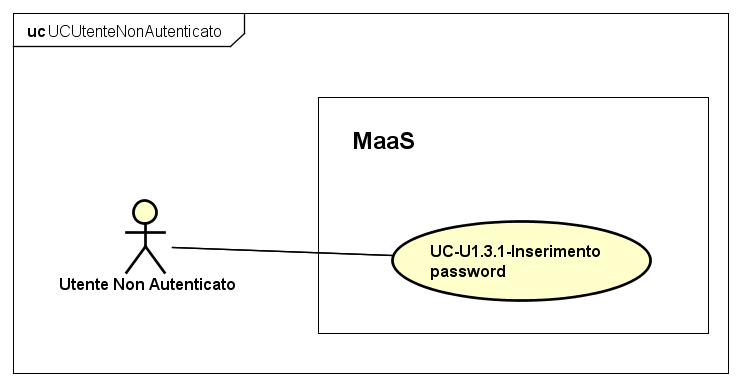
\includegraphics[width=12cm]{res/img/UCUtenti/UCUtenteNA/UC-U1.3-Registrazione Azienda/UC-U1.3-RegistrazioneAzienda}
      \caption{UC-U1.3 - Registrazione Azienda}
      \end{center} 
    \end{figure}    
    
    %Tabella 
    \begin{center}
      \bgroup
      \def\arraystretch{1.8}     
      \begin{longtable}{  p{3.5cm} | p{8cm} } 
        
        \hline
        \multicolumn{2}{ | c | }{ \cellcolor[gray]{0.9} \textbf{UC-U1.3 - Registrazione Azienda}} \\ 
        \hline
        
        \textbf{Attori Primari} & Utente non autenticato \\ 
        \textbf{Scopo e Descrizione} & L'utente non autenticato inserisce la password associata all'account della propria azienda. \\ 
        
        \textbf{Precondizioni}  & L'utente non autenticato ha visualizzato la pagina per la registrazione dell'azienda. \\ 
        
        \textbf{Postcondizioni} & L'utente non autenticato ha inserito una password associata all'account dell'azienda. \\ 
        \textbf{Flusso Principale} & 1. L'utente non autenticato inserisce una password associata all'account dell'azienda. \\
        \textbf{Estensioni} & Nessuna \\
        \textbf{Inclusioni} & Nessuna \\
      \end{longtable}
      \egroup
    \end{center}
    
\subsubsection{UC-U3}

    \begin{figure}[H]
      \begin{center}
        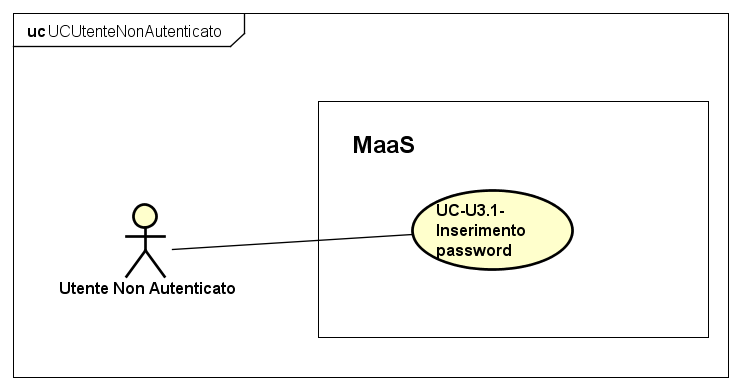
\includegraphics[width=12cm]{res/img/UCUtenti/UCUtenteNA/UC-U3-Registrazione Utente/UC-U3-RegistrazioneUtente}
      \caption{UC-U3 - Registrazione Utente}
      \end{center} 
    \end{figure}    
    
    %Tabella 
    \begin{center}
      \bgroup
      \def\arraystretch{1.8}     
      \begin{longtable}{  p{3.5cm} | p{8cm} } 
        
        \hline
        \multicolumn{2}{ | c | }{ \cellcolor[gray]{0.9} \textbf{UC-U3 - Registrazione Utente}} \\ 
        \hline
        
        \textbf{Attori Primari} & Utente non autenticato \\ 
        \textbf{Scopo e Descrizione} & L'utente non autenticato può registrarsi su MaaS. \\ 
        
        \textbf{Precondizioni}  & L'utente non autenticato è in possesso di un account valido. \\ 
        
        \textbf{Postcondizioni} & L'utente non autenticato ha creato un account valido presso MaaS e può effettuare il login. \\ 
        \textbf{Flusso Principale} & 1. L'utente inserisce la propria password (UC-U3.1) \\
        \textbf{Estensioni} & Nessuna \\
        \textbf{Inclusioni} & Nessuna \\
      \end{longtable}
      \egroup
    \end{center} 

\subsubsection{UC-U4}

    \begin{figure}[H]
      \begin{center}
        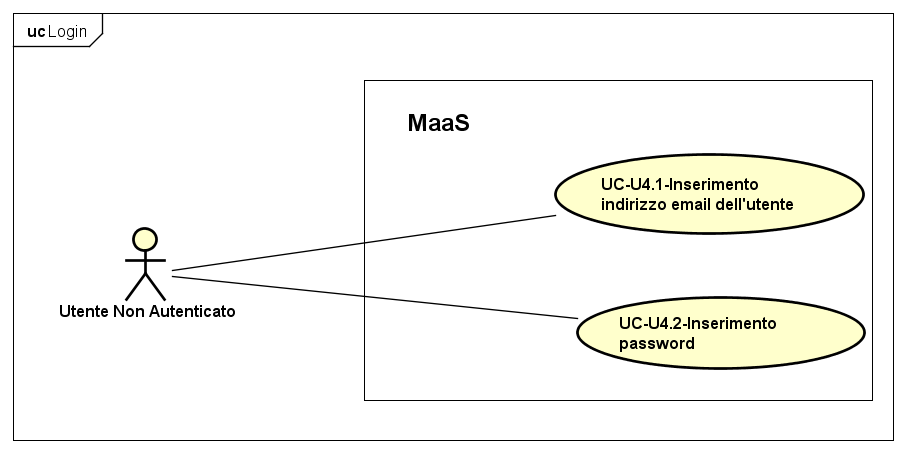
\includegraphics[width=12cm]{res/img/UCUtenti/UCUtenteNA/UC-U4-Login/UC-U4-Login}
      \caption{UC-U4 - Login}
      \end{center} 
    \end{figure}    
    
    %Tabella 
    \begin{center}
      \bgroup
      \def\arraystretch{1.8}     
      \begin{longtable}{  p{3.5cm} | p{8cm} } 
        
        \hline
        \multicolumn{2}{ | c | }{ \cellcolor[gray]{0.9} \textbf{UC-U4 - Login}} \\ 
        \hline
        
        \textbf{Attori Primari} & Utente non autenticato \\ 
        \textbf{Scopo e Descrizione} & L'utente non autenticato può effettuare il login all'applicazione. \\ 
        
        \textbf{Precondizioni}  & L'utente non autenticato è in possesso di un account valido. \\ 
        
        \textbf{Postcondizioni} & L'utente non autenticato diventa un utente autenticato e ha accesso alle funzionalità di MaaS concesse dalla tipologia di account (ruolo). \\ 
        \textbf{Flusso Principale} & 1. L'utente non autenticato inserisce il proprio indirizzo email (UC-U4.1)
        
2. L'utente non autenticato inserisce la password (UC-U4.2) \\
        \textbf{Estensioni} & Nessuna \\
        \textbf{Inclusioni} & Nessuna \\
      \end{longtable}
      \egroup
    \end{center} 
    
\subsubsection{UC-U4.1}  
   
    %Tabella 
    \begin{center}
      \bgroup
      \def\arraystretch{1.8}     
      \begin{longtable}{  p{3.5cm} | p{8cm} } 
        
        \hline
        \multicolumn{2}{ | c | }{ \cellcolor[gray]{0.9} \textbf{UC-U4.1 - Inserimento indirizzo email dell'utente}} \\ 
        \hline
        
        \textbf{Attori Primari} & Utente non autenticato \\ 
        \textbf{Scopo e Descrizione} & L'utente non autenticato inserisce il proprio indirizzo email. \\ 
        
        \textbf{Precondizioni}  & L'utente non autenticato è in possesso di un account valido. \\ 
        
        \textbf{Postcondizioni} & Il campo testo \`e stato compilato con il contenuto richiesto. \\ 
        \textbf{Flusso Principale} & Nessuno \\
        \textbf{Estensioni} & Nessuna \\
        \textbf{Inclusioni} & Nessuna \\
      \end{longtable}
      \egroup
    \end{center} 

\subsubsection{UC-U4.2}
    
    %Tabella 
    \begin{center}
      \bgroup
      \def\arraystretch{1.8}     
      \begin{longtable}{  p{3.5cm} | p{8cm} } 
        
        \hline
        \multicolumn{2}{ | c | }{ \cellcolor[gray]{0.9} \textbf{UC-U4.2 - Inserimento password utente}} \\ 
        \hline
        
        \textbf{Attori Primari} & Utente non autenticato \\ 
        \textbf{Scopo e Descrizione} & L'utente non autenticato inserisce la password associata al proprio account. \\ 
        
        \textbf{Precondizioni}  & L'utente non autenticato è in possesso di un account valido. \\ 
        
        \textbf{Postcondizioni} & Il campo testo \`e stato compilato con il contenuto richiesto. \\
        \textbf{Flusso Principale} & Nessuno \\
        \textbf{Estensioni} & Nessuna \\
        \textbf{Inclusioni} & Nessuna \\ 
      \end{longtable}
      \egroup
    \end{center} 

\subsubsection{UC-U6}

    \begin{figure}[H]
      \begin{center}
        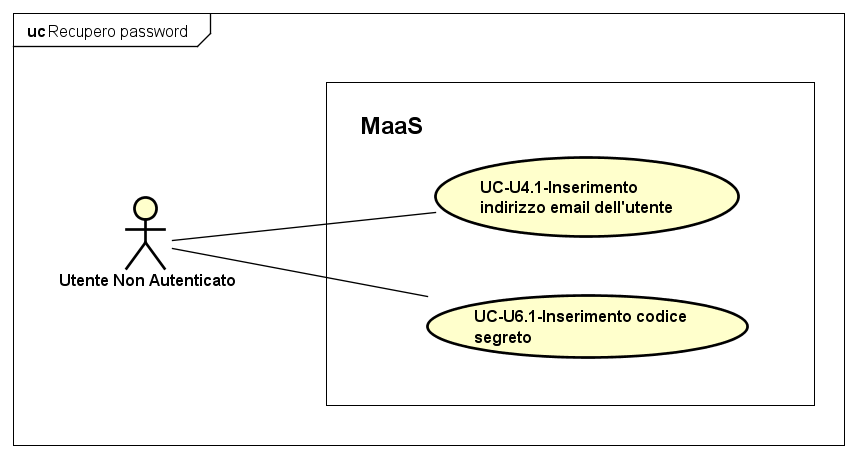
\includegraphics[width=12cm]{res/img/UCUtenti/UCUtenteNA/UC-U6-Recupero Password/UC-U6-RecuperoPassword}
      \caption{UC-U6 - Recupero password}
      \end{center} 
    \end{figure}    
    
    %Tabella 
    \begin{center}
      \bgroup
      \def\arraystretch{1.8}     
      \begin{longtable}{  p{3.5cm} | p{8cm} } 
        
        \hline
        \multicolumn{2}{ | c | }{ \cellcolor[gray]{0.9} \textbf{UC-U6 - Recupero password}} \\ 
        \hline
        
        \textbf{Attori Primari} & Utente non autenticato \\ 
        \textbf{Scopo e Descrizione} & L'utente non autenticato effettua la procedura per il recupero della password, inserendo il proprio indirizzo email e il codice segreto che gli verrà inviato. \\ 
        
        \textbf{Precondizioni}  & L'utente non autenticato è in possesso di un account. \\ 
        
        \textbf{Postcondizioni} & L'utente non autenticato ha ottenuto una nuova password per accedere a MaaS. \\ 
        \textbf{Flusso Principale} & 1. L'utente non autenticato inserisce il proprio indirizzo email (UC-U4.1)
        
2. L'utente non autenticato inserisce il codice segreto ricevuto (UC-U4.2) \\
        \textbf{Estensioni} & Nessuna \\
        \textbf{Inclusioni} & Nessuna \\
      \end{longtable}
      \egroup
    \end{center} 

\subsubsection{UC-U6.1} 
    
    %Tabella 
    \begin{center}
      \bgroup
      \def\arraystretch{1.8}     
      \begin{longtable}{  p{3.5cm} | p{8cm} } 
        
        \hline
        \multicolumn{2}{ | c | }{ \cellcolor[gray]{0.9} \textbf{UC-U6.1 - Inserimento codice segreto}} \\ 
        \hline
        
        \textbf{Attori Primari} & Utente non autenticato \\ 
        \textbf{Scopo e Descrizione} & L'utente non autenticato inserisce il codice segreto ricevuto tramite email mentre stava effettuando la procedura di  recupero della password. \\ 
        
        \textbf{Precondizioni}  & L'utente non autenticato  ha inserito correttamente il proprio indirizzo email durante la procedura di recupero della password. \\ 
        
        \textbf{Postcondizioni} & Il campo testo \`e stato compilato con il contenuto richiesto. \\ 
        \textbf{Flusso Principale} & Nessuno \\
        \textbf{Estensioni} & Nessuna \\
        \textbf{Inclusioni} & Nessuna \\
      \end{longtable}
      \egroup
    \end{center} 

    
